
%(BEGIN_QUESTION)
% Copyright 2010, Tony R. Kuphaldt, released under the Creative Commons Attribution License (v 1.0)
% This means you may do almost anything with this work of mine, so long as you give me proper credit

Combine any relevant formulae for series resistor circuits to create a new formula calculating the power dissipation of $R$, given the other values (constants) in this circuit and the resistance value $R$:

$$\includegraphics[width=15.5cm]{i03230x01.eps}$$

Your answer should be in fully-expanded form (no parentheses or compound fractions).  Be sure to show all your work!

\vskip 40pt

$P_R = $

\vfil 

\underbar{file i03230}
\eject
%(END_QUESTION)





%(BEGIN_ANSWER)

This is a graded question -- no answers or hints given!

%(END_ANSWER)





%(BEGIN_NOTES)

First, we will begin with a formula known to solve for power through a resistance $R$:

$$P_R = I^2 R$$

\vskip 10pt

Next, we will substitute an expression of Ohm's Law $\left( I = {V \over R} \right)$ based on total voltage and total series resistance into that power formula:

$$P_R = \left({12 \over {1200 + R}}\right)^2 R$$

\vskip 10pt

From here on out, we just square the current term and use algebra to simplify the expression:

$$P_R = {{144 R} \over {1440000 + 2400R + R^2}}$$

%INDEX% Mathematics review: substituting equations

%(END_NOTES)


